\section{Data Observation: A Pilot Study on the Stress-buffering Effect of School Scheduled Positive Events}
\label{sec:obs}
\paragraph{Microblogs} Microblogs of students coming from Taicang High School were collected from January 1st, 2014 to September 1st, 2017.
We filtered out 121 active students according to their posting frequency from over 500 students,
and collected their microblogs throughout the whole high school career.
Totally 27,346 microblogs were collected in this research,
where 226 microblogs per student on average, 1,421 microblogs maximally and 102 posts minimally.
To protect the privacy, all usernames were anonymized during the experiment.

\paragraph{Scheduled events} The list of weekly scheduled school events,
with detailed description involved in the event (grade, exact start and end time),
were collected from the school's official website\footnote{http://stg.tcedu.com.cn/col/col82722/index.html} from February 1st, 2014 to August 1st 2017.
There were 126 stressor events and 75 positive events in total.
Examples of scheduled positive and stressor events in high school life are listed shown in Table~\ref{tab:example}.
There were 2-3 stressor events and 1-2 positive event scheduled per month in current study.
Figure~\ref{fig:example} shows three examples of a student's stress fluctuation during three mid-term exams,
where the positive event \emph{campus art festival} was scheduled ahead of the first exam (\emph{example a}),
the positive event \emph{holiday} happened after the second exam (\emph{example b}),
and no scheduled positive event was found nearby the third exam (\emph{example c}).


\begin{table}[H]
\caption{\small{Examples of school scheduled positive and stressor events.}}
\label{tab:example}
\resizebox{.45\textwidth}{9mm}{
\small{
\begin{tabular}{cccc}
\toprule
Type & Date	& Content	& Grade	\\
\midrule
stressor event & 2017/4/16 & first day of mid-term exam & grade1,2\\
positive event & 2016/11/5 & campus art festival & grade1,2,3\\
\bottomrule
\end{tabular}
}
}
\end{table}

\begin{table}[h]
\centering
\caption{\small{Examples of academic related keywords.}}
\label{tab:studyWords}
\small{
\begin{tabular}{c}
\toprule
exam, fail, review, score, test paper, rank, pass, math, chemistry\\
homework, regress, fall behind, tension, stressed out, physics,\\
nervous, mistake, question, puzzle, difficult, lesson, careless\\
\bottomrule
\end{tabular}
}
\end{table}


\begin{figure}[H]
\centering
\includegraphics[width=\linewidth]{figs/exampleWave.eps}
\caption{\small{Examples of school scheduled positive events, stressor events, and a student's stress fluctuation}}
\label{fig:example}
\end{figure}

To further observe the effect of positive events on stressed students,
we collected all stressful intervals surround the scheduled exams over the 121 students during their high school career
applying the interval detection method in ~\citep{Li2017Analyzing}.
For each student, we divided all stressful intervals into two sets:
1) In the original sets, stress was caused by a stressor event, lasting for a period,
and no other intervention (namely, positive event) occured.
We called the set of such stressful intervals as \textbf{SI};
2) In the other comparative sets,
the stressful interval was impacted by a positive event,
we called the set of such stressful intervals as \textbf{U-SI}.
Thus the difference under the two situations (sets) could be seen as the stress-buffering effect
conducted by the positive event.
We identified 518 exam related stressful intervals (SI)
and 259 stressful intervals impacted by four typical scheduled positive events (U-SI)
('practical activity', 'new year party', 'holiday', 'sports meeting') from the students' microblogs.
Six measures in the above two conditions were considered:
the \emph{accumulated value of stress}, the \emph{average value of stress} (per day),  the \emph{maximal value of stress} (per day),
the \emph{RMS value of stress},
the \emph{frequency of academic topic words}, and the \emph{ratio of academic stress among all types of stress}.
Since our target was to track the impact of positive events for students under stress,
based on previous research~\cite{XueUbicomp13},
we detected the stress level (ranging from 0 to 5) for each post.
For each student,
the stress value per day was aggregated by calculating the average stress of all posts.
Examples of academic related keywords were listed in table \ref{tab:studyWords}.
The average value of each measure over all eligible slides was calculated.


\begin{figure}[h]
\centering
%\includegraphics[width=0.8\linewidth]{figs/obnew-color.eps}
\includegraphics[width=\linewidth]{figs/barUSI.eps}
\caption{\small{Comparing stress (average value of all students) during exam intervals in two situations:
1) intervals affected by neighboring positive events (U-SI), 2) no positive events occurred nearby (SI).}}
\label{fig:frequency}
\end{figure}

\paragraph{Results}
As shown in figure~\ref{fig:frequency},
comparing each measure of scheduled exam intervals under the two situations:
1) existing neighbouring positive events (U-SI) and 2) no neighbouring scheduled positive events (SI),
we found that students during exams with neighbouring positive events exhibited less stress intensity
(78.13\% reduction in average stress, 95.58\%  reduction in cumulative stress, xx\%  reduction in maximal stress)
and more stable stress fluctuations (xx\% reduction in RMS values of stress).
%and shorter duration of stress intervals (23.30\% reduction).
Further, the frequency of academic topic words (table \ref{tab:studyWords} for examples)
and the ratio of academic stress in each interval were calculated.
Most students talked less about exams when positive events happened nearby,
with lower frequency (84.65\% reduction) and lower ratio (89.53\% reduction).
The statistic result shows clues about the impact of scheduled positive events,
which is constant with the psychological theory ~\citep{Cohen1984Positive, Cohen2010Positive, Needles1990Positive},
indicating the reliability and feasibility of the microblog data set.
However,
this is an observation based on specific scheduled events,
and cannot satisfy the need for automatic, timely, and continuous perception of stress-buffering process.
Therefore, next, we will propose a framework to automatically detect positive events and its impact interval.
Based on this,
the relationship between the impact of automatically extracted positive events
and adolecents' microblogging characteristics will be discussed.


\begin{figure}
\centering
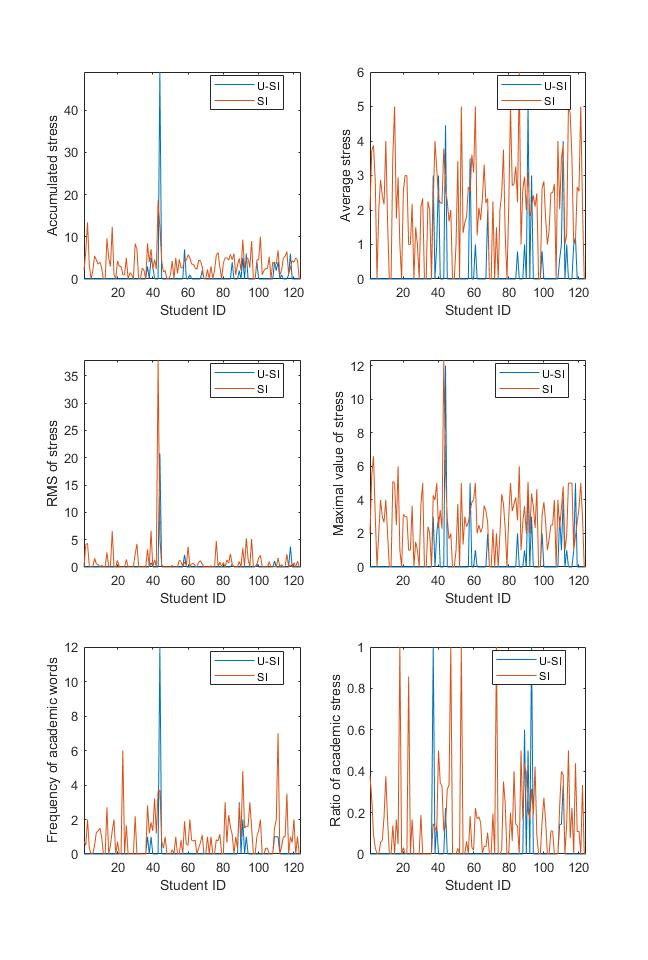
\includegraphics[width=\linewidth]{figs/activity.eps}
\caption{\small{Comparing students' stress during exam intervals in two situations:
1) intervals affected by practical activities (U-SI), 2) no positive events occurred nearby (SI)}}
\label{fig:frequency}
\end{figure}
